\scanpage{111}
\mspage{54}

\deleted{on which $\Sigma$ operates} \inserted{and the operation of $\Sigma$} \deleted{\unsure{on it}} on $\pi$ is
compatible with this loop structure,
and the cyclotomic character $\chi:\Gamma\to\widehat{\mathbb Z}^{*}$
(\unsure{rather}, $\chi\mid\Sigma$). Thus the operation of
$\Sigma$ on $\pi$ implies its action on $I$, whence
$S(\overline K)\simeq\unsure{I_0|\overline S_0}\wedge_{\Sigma}\Gamma$ as a $\Sigma$-set
--- we thus recover the étale $K$-scheme $S$.

But better, we recover the whole
diagram
\diagram{\begin{tikzcd}[ampersand replacement=\&]
\Pi_{\overline D_0^{*}} \arrow[r] \& {[\Pi_{\overline U_0}\unsure{\to|-}]}\,\Pi_{\overline U} \arrow[r] \& \Pi_e
\end{tikzcd}}
and the operation of $\Sigma$ on it, whence the
diagram of topoi \unsure{of coverings}\inserted{\deleted{``\unsure{classifying|étale}'' \illegible{1}}} --- or if
we prefer, the diagram
\diagram{\begin{tikzcd}[ampersand replacement=\&]
\Pi_{D^{*}} \arrow[r] \& \Pi_U \arrow[r] \& \Pi_e
\end{tikzcd}}
(with the notation from the beginning of these notes,
which here would become $\Pi_{D^{*},\Gamma}\to\Pi_{U,\Gamma}\to\Pi_{e,\Gamma}$),
plus of course $K$\dots

The morphisms $(X',S')\xrightarrow{f}(X,S)$
[$S'\supset f^{-1}(S)$, $f$ dominant] \deleted{\unsure{correspond}} \inserted{are described}
\deleted{\unsure{simply to the}} \inserted{simply} (via the choice of an $\overline X'_0$
over an $\overline X_0$) \deleted{to the} \inserted{by} outer homomorphisms

\margin{\uline{\unsure{(159)}}}
\margin{110}

\scanpage{112}

$\pi'\deleted{\unsure{\illegible{1}}}\ (=\pi_1(\overline X'_0))\longrightarrow\pi\ (=\pi_1(\overline X_0))$, compatible
with the actions of $\Sigma'\ (\subset\Sigma)$ and of $\Sigma$,
and with the anabelian loop structures
(which is expressed \deleted{by} \inserted{with the aid of} a map
$\tau:I'\subset\overline S'_0\deleted{\illegible{1}}\longrightarrow I=\overline S_0$ compatible with
$\Sigma'$, and a system of natural numbers
$(d_i)_{i\in I'}$).
\margin{\uline{N.B.} $I'=\overline S'_0\cap f^{-1}(\overline S_0)$}

We must however complete, \deleted{\illegible{1}} for
$I=\varnothing$ i.e. $S=\varnothing$, the definition of the
loop structure, by the datum of an
isomorphism
\[
\kappa:T^{\otimes-1}\simeq H^2(\pi,\widehat{\mathbb Z})
\]
[N.B., in characteristic $p\geq0$, we must restrict ourselves
to the $l$-adic components with $l\ne p$]
i.e.
\[
\widehat{\mathbb Z}\simeq H^2(\pi,T)
\]
compatible with the action of $\Sigma$
--- and we must require, in the
``Galoisian'' interpretation of $f:(X',S')\unsure{\to}(X,S)$, when $S=S'=\varnothing$
that the homomorphism $\pi\to\pi'$ induces a
commutative diagram

\margin{111}

\scanpage{113}
\mspage{55}

\diagram{\begin{tikzcd}[ampersand replacement=\&]
\widehat{\mathbb Z} \arrow[r, no head, "\unsure{\kappa^{*}|\kappa}", "\sim"'] \arrow[d, "d"'] \& H^2(\unsure{\pi},T) \arrow[d, "f^{*}"] \\
\widehat{\mathbb Z} \arrow[r, "\kappa'", "\sim"'] \& H^2(\pi',T)
\end{tikzcd}},
where $d$\inserted{$(\in\mathbb N)$} is the \uline{degree} (defined \deleted{\unsure{in terms}} \inserted{uniquely}
by this condition,
\deleted{Galoisian} \unsure{as|or also} \inserted{\unsure{but}} the order of $\operatorname{Coker}f^{*}$). \deleted{\illegible{1}}

\deleted{a priori we would thus have} \inserted{When $\unsure{S^{*}|S}=\varnothing$, $\unsure{S'|S'_0}\ne\varnothing$, there should be}
still be a compatibility
for the Kummerian data (of
\unsure{different natures|a different nature} on $\pi'$, where there really are
``loops'', and on $\pi$, where it is
purely cohomological\unsure{)|s}. \unsure{\S} The question
is probably equivalent to that of describing
a ``cohomological'' Kummerian structure
on the group $\widetilde\pi'$, obtained from a $\pi'$ with
loops (with $I'\ne\varnothing$) by dividing by
the said loops. The question is the
same, it seems, in the topological setting,
or the arithmetic setting, I shall have to
come back to it. It would be necessary that for \unsure{every}

\margin{paradigm of the passage from $(X,S)$ to $X$ : ``plugging the holes''\dots}
\margin{112}

\scanpage{114}

homomorphism \inserted{$\pi'\to\pi$} of groups with $T$-loops, the corresponding homomorphism
$\unsure{\widehat\pi'|\widetilde\pi'}\to\widetilde\pi$ also respect (for
a suitable degree) the loop structure.

When we are interested \deleted{in the} anabelian systems
$(\overline X,\overline S)$ defined directly \uline{over $\overline K$}, with $\overline X$
connected say, this is expressed
by an outer group with $T$-loops,
endowed with an action (not of $\Gamma$ but
of the) profinite group \uline{kernel} defined by $\Gamma$.
If we consider the \deleted{\illegible{1}} ``$\Gamma$-automorphisms'' of
such an object (formed of a $\gamma\in\Gamma$ and
an \inserted{outer} automorphism $f$ of $\pi$ respecting the
loop structure, $f$ and $\gamma$ being compatible
in an obvious sense\dots), we find
a group \inserted{\deleted{profinite} (pro-finite ???)} $G$ and a homomorphism \inserted{(``discrete'' ???)} $G\to\Gamma$
with image an open subgroup of $\Gamma$, and
with kernel \inserted{$G_0$} the group of \unsure{Galois|outer} loop automorphisms of $\pi$ which commute with the action \unsure{of the|of the}
\inserted{``kernel''}\deleted{\illegible{1}} \deleted{\unsure{typical}} (which $G_0$ is conjecturally by the
``messy conjecture'', isomorphic to \inserted{to the finite group} $\operatorname{Aut}_{\overline K}(\overline X,\overline S)$\dots).

\margin{113}

\scanpage{115}
\mspage{56}

In terms of this exact sequence
\[
1\unsure{\longrightarrow|-}G_0\longrightarrow G\unsure{\longrightarrow|-}\Gamma
\]
the ``restriction of $(\overline X,\overline S)$ to the field $K$'' is
therefore expressed (we hope, in a fully faithful way,
if the messy conjecture is valid) by
a splitting $\Gamma\to G$ of $G\to\Gamma$\dots

$13^{\mathrm{bis}}$. \uline{Return to the notion of group with loops}

Let $\pi$ be a group, $([L_i])_{i\in I}$ a family
of conjugacy classes of subgroups of
$\pi$. We say that this defines a \deleted{\unsure{some}}
``loop structure'' on $\pi$ \inserted{[of type $(g,\nu)$]}, if $\exists\,g\in\mathbb N$,
\unsure{\deleted{$\forall i\in I$}|$\forall i\in I$} an $L_i\in[L_i]$, a generator
$l_i\in L_i$, elements $\unsure{x_\alpha},y_\alpha\in\pi$ $(1\le\alpha\le g)$
finally an order $i_1\dots i_\nu$ on $I$ (\deleted{of} \inserted{$\nu=$} cardinality$(I)$),
such that (putting $l_\alpha=l_{i_\alpha}$ for simplicity)
\[
[x_1,y_1][x_2,y_2]\dots[x_g,y_g]l_1\dots l_\nu=0
\]
\unsure{is|are} a presentation of the \uline{group} $\pi$. We
do not exclude a priori either the case $g=0$, or the case $\nu=0$,
i.e. $I$ empty.

We deduce from this:

a) If $\nu\ne0$, $\pi$ is free (on $2g+\nu-1$ generators) ---
hence free \uline{nonabelian} unless $g=0$, $\nu\le2$ \deleted{\illegible{1}}.

\margin{114}

\scanpage{116}

b) If $\nu=0$, the only case where $\pi$ abelian is the one
$g\le1$. [Thus $\pi\simeq\pi_{g,\nu}$ is abelian iff
$g=0$, $\nu\le3$ or $g=1$, $\nu\unsure{\le|=}0\deleted{\unsure{\text{or }1}}$]
\margin{\unsure{To say that|Although} \deleted{\illegible{1}} $\pi=0$ \deleted{\illegible{1}}) \deleted{\illegible{2}} $g=0$, $\nu=0,1$, \unsure{and outside these cases} the $L_i$ \unsure{are} $\simeq\mathbb Z$.}

In any case, we have a canonical exact sequence
of free $\mathbb Z$-modules of finite type
\[
0\unsure{\longrightarrow|-}T_\pi\longrightarrow\prod_{i\in I}L_i
\xrightarrow{i}\pi_{\mathrm{ab}}\unsure{\longrightarrow|-}\widetilde\pi_{\mathrm{ab}}\longrightarrow0
\]
\margin{\uline{N.B.} Unless $\pi=0$, i.e. $g=0$, $\nu=0,1$, the $L_i$ are $\simeq\mathbb Z$.}
where, \inserted{for $I\ne\varnothing$, $\pi\ne0$} $T_\pi$ is $\simeq\mathbb Z$ (defined as $\operatorname{Ker}i$), and where
the projections
\[
T_\pi\longrightarrow L_i
\]
are isomorphisms. In the case $I\ne\varnothing$, we
call $T_\pi$ the \uline{$\mathbb Z$-module of orientations of}
$\pi$ (endowed with the family of $(L_i)$) ---
we define, \deleted{more \illegible{1} $T_\pi$ \unsure{if} $I$ \illegible{2}} \inserted{if $I=\varnothing$, $(\nu=0)$, but $g\ne0$}
(so $\pi\ne1$ --- the only case $\pi=1$ is that where
$g=0$, $\nu=0$ or $1$) by the condition
\[
T_\pi=\underbrace{H^2(\pi,\mathbb Z)}_{\substack{\mathbb Z\text{-module}\\\text{free of rank }1}}{}^{\otimes-1}
\]
[we shall establish below a relation between the
two definitions of $T_\pi$]. Thus $\pi_{\mathrm{ab}}$
is \inserted{free} of rank $2g+\nu-1$ if $\nu\ne0$, $2g$ if $\nu=0$.
(so $g$ is uniquely determined by $\pi$ and $\nu=\operatorname{card}I$.
\deleted{the family of $([L_i])$.}

\margin{115}

\scanpage{117}
\mspage{57}

Note that [if $\nu\ne0$, \inserted{and]} except for the ``abelian''
cases $g=0$, $\nu=1,2$, the conjugacy classes
of the $L_i$ $(i\in I)$ are distinct, so the
loop structure of $\pi$ can be described
as the datum of a set of $\nu$ conjugacy
classes of subgroups of $\pi$. Moreover,
\deleted{(from the fact that $L_i\to\pi_{\mathrm{ab}}$ injective}
we see that $\forall\,g\in\pi$ which normalizes
an $\unsure{L_i}$ centralizes it (this is obvious
in any case for $\nu\ge2$, for then
$L_i\to\pi_{\mathrm{ab}}$ is injective), which implies
that the $\{L_i\}$ of one and the same class $[L_i]$
are canonically isomorphic to one another
\deleted{(\illegible{1} \unsure{isomorphic} :}
which gives an intrinsic meaning to the
term $\prod L_i$ in the exact sequence
above, and to the canonical isomorphism $T_\pi\to L_i$\dots
\margin{see separately the case $\nu=1$ : normalizer of the subgroup generated by $\prod[x_\alpha,y_\alpha]$, in the free group generated by the generators $x_\alpha,y_\alpha$\dots}

If a group $\Sigma$ operates on the loop
structure $(\pi,([L_i]))$ it operates on the
invertible $\mathbb Z$-module $T_\pi$, whence a
character
\[
\chi:\Sigma\longrightarrow\mathbb Z^{*}=\{\pm1\}
\]
---
\margin{We assume from now on that we are in the anabelian case, or at least, we exclude $g=0$, $\nu\le2$}

\margin{116}

\scanpage{118}

conversely, if we have a character \inserted{$\chi$ on $\Sigma$} given in advance,
we shall speak of an \deleted{\illegible{1}}action of $\Sigma$ on $(\pi,([L_i]))$
\uline{compatible} with $\chi$. If we are given an
invertible $\mathbb Z$-module $T$, a $T$-loop structure
on a group with loops $\pi$ (with $\pi\ne0$), endowed
with an isomorphism $T\simeq T_\pi$, \deleted{and if $\Sigma$ operates on
$T$ (\illegible{3} $\chi$), we shall say that an action
is compatible}

We have profinite variants
(or prime-to-$p$ profinite ones, if $p$ is a given
prime\dots) --- but already now there are
two points to note, to be checked in
this case:
\[
\left\{
\begin{array}{l}
\operatorname{Norm}_{\pi}(L_i)=\operatorname{Centr}_{\pi}(L_i)=L_i
\ \inserted{\text{in the}}\ \text{case }\nu=1,\ \inserted{\text{otherwise no problem}}\\[4pt]
\operatorname{Centr}(\pi)=(1)\quad(\text{anabelian case})
\end{array}
\right.
\]
more generally, the centralizer
of \unsure{every} open subgroup of $\pi$
is reduced to $1$\dots
\margin{This is not \uline{proved} for the moment in \uline{any} profinite anabelian case!}

\figure{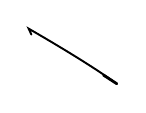
\begin{tikzpicture}[x=1cm,y=1cm,line cap=round]
\draw[line width=0.7pt] (0.035,-0.075) -- (0,0) .. controls (0.33,-0.19) and (0.80,-0.47) .. (1.12,-0.70);
\draw[line width=1.0pt] (0.95,-0.59) -- (1.12,-0.70);
\end{tikzpicture}}
\margin{117}

\scanpage{119}
\mspage{58}

14. Cohomological digression (on \unsure{the|the} ``plugging the
holes).

Let $X$ be a locally noetherian \uline{regular} scheme of
\unsure{dimension} $1$, $S$ a closed subscheme \inserted{reduced discrete} such that
$\forall s\in S$, $\dim_s S=1$ (so $S$ defined by a
closed discrete subset of $X$), $U=X\setminus S$.
\margin{It might perhaps be better to start with \unsure{the purely topological case|the purely topological cases} of a surface\dots{} and make the link with \uline{discrete} groups.}

We want to make explicit by Galoisian means the
étale sheaves \inserted{of sets} \inserted{constructible} on $X$ such that $F\mid U$ is
locally constant. By the \unsure{topos|carpet} of Artin \inserted{on the opens of the topos}, they
correspond to triples
\[
(F_U,F_S,\varphi)
\]
where $F_U$ is a \inserted{constructible} locally constant sheaf on $U$,
$F_S$ a sheaf (\unsure{necessarily|necessarily} locally constant)
and $\varphi$ a morphism
\[
F_S\xrightarrow{\varphi}j^{*}i_{*}(F_U)
\]
(where $i:U\unsure{\hookrightarrow|\to}X$ and $j:S\to X$ are the inclusions).
Any constructibility condition being set
aside, an étale sheaf $F$ on $X$ corresponds
to such a triple --- we restrict ourselves here to the
$F$ such that $F_U$ \deleted{\unsure{comes}} comes from the
fundamental topos $B_{\unsure{\Pi_1(U)|\pi_1(U)}}$ of $U$ \deleted{\illegible{1}}\dots
(There is no need to assume $F_U$ has finite fibers,

\margin{118}

\scanpage{120}

for what follows). \deleted{We are going to}

Let $\forall s\in S$ $\underline{O}_s$ be a henselization of $\underline{O}_{X,s}$,
$D_s=\operatorname{Spec}\underline{O}_s$ \inserted{(``disk at $s$'')}, $D_s^{*}=D_s-\{s\}$ \inserted{$=\operatorname{Spec}K_s$ ($K_s$ field of fractions of $\underline{O}_s$)} (``pointed disk'' at
$s$) $D=\coprod_{s\in S}D_s$, $\unsure{D_s^{*}|D^{*}}=\coprod_{s\in S}D_s^{*}$. We have
a commutative diagram
\diagram{\begin{tikzcd}[ampersand replacement=\&]
\& D^{*} \arrow[dl, "\rho"'] \arrow[dr, "\sigma"] \& \& \\
U \arrow[dr, "i"'] \& \& D \arrow[dl, "\unsure{k|\kappa}"] \& S \arrow[l, dashed, "j_0"'] \arrow[dll, dashed, "j"] \\
\& X \& \&
\end{tikzcd}
[The dotted branch $S\xrightarrow{j_0}D$ is placed in parentheses.]}
and we see \inserted{(by Artin)} that this diagram \deleted{\unsure{makes of}} \inserted{allows us to express}
\inserted{the sheaves} \deleted{topoi} étale on $X$ \deleted{\unsure{as amalgamated}}
\deleted{of the étale topoi of $U,D$ over $D^{*}$}
\deleted{\diagram{\begin{tikzcd}[ampersand replacement=\&,column sep=2.5em,row sep=2em,nodes in empty cells]
\& \deleted{\unsure{D^*_{\mathrm{\acute et}}}} \arrow[dl] \arrow[dr] \& \\
\deleted{U_{\mathrm{\acute et}}} \& \& \deleted{D_{\mathrm{\acute et}}}
\end{tikzcd}}}
as systems \deleted{of sheaves} \inserted{$(F_U,F_D,\varphi)$}
with $F_U$ an étale sheaf on $U$, $F_D$ an étale
sheaf ``essential\textsuperscript{ly} locally constant'' on $D$ [N.B. the
inclusion $S\to D$ defines an equivalence
between the category of these sheaves on $D$, and
that of étale sheaves on $S$] and
a morphism of sheaves $F_D\to\sigma_{*}\rho^{*}F_U$ or again

\margin{119}
